\documentclass[12pt,a4paper]{article}
\usepackage[utf8]{inputenc}
\usepackage[portuguese]{babel}
\usepackage{amsmath}
\usepackage{amsfonts}
\usepackage{amssymb}
\usepackage{enumitem}
\usepackage{geometry}
\usepackage{graphicx}
\usepackage{multicol}
\usepackage{tcolorbox}
\usepackage{setspace}
\setstretch{1.2}
\tcbuselibrary{skins} 
\usepackage{pgfplots}
\pgfplotsset{compat=1.15}
\usepackage{mathrsfs}
\usepackage{tasks}
\usepackage{tikz}
\usetikzlibrary{calc}
\usetikzlibrary{arrows, intersections, angles, calc, quotes, babel}

\geometry{top=2cm, bottom=2cm, left=2.5cm, right=2.5cm}

\begin{document}
	
	% --- CABEÇALHO COM CAIXA ---
	\begin{tcolorbox}[
		enhanced, 
		colback=white, 
		colframe=black, 
		boxrule=2pt,
		left=0pt, 
		right=0pt,
		top=5pt,
		bottom=5pt
		]
		\noindent
		\begin{minipage}[c]{0.24\linewidth}
			\centering
			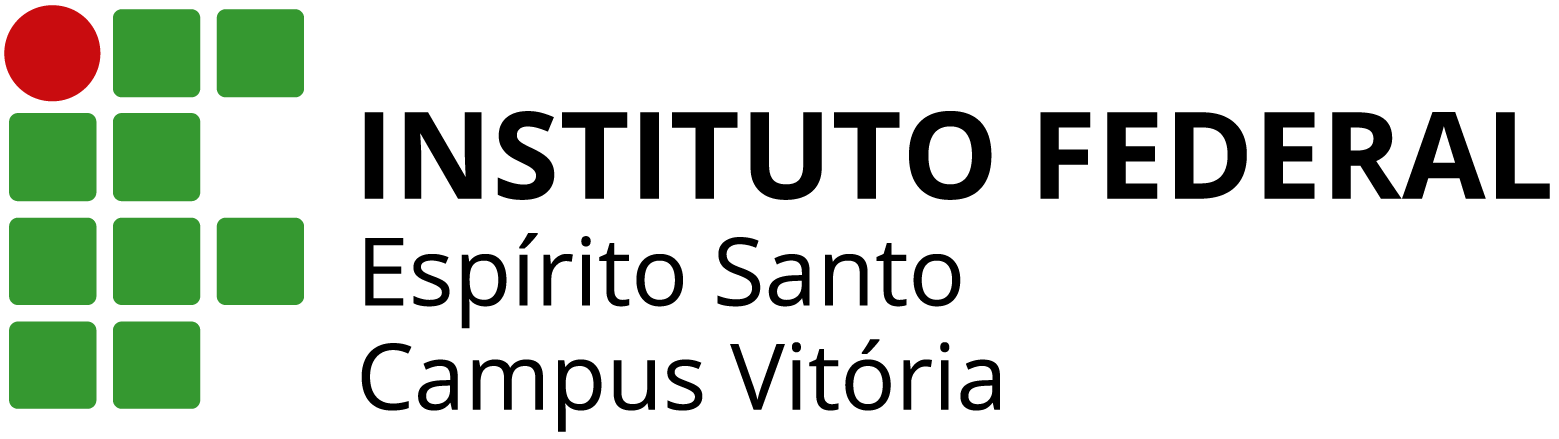
\includegraphics[width=0.9\linewidth]{ifes.png} 
		\end{minipage}%
		\begin{minipage}[c]{0.51\linewidth}
			\centering
			\textbf{Debates Conceituais Avançados em Matemática -- 2026/2}\\
			\textbf{Doutorado Educimat}\\
			\textbf{Razão Áurea e Sequência de Fibonacci}\\	
			Professor: \textbf{Alex Jordane}
		\end{minipage}%
		\begin{minipage}[c]{0.24\linewidth}
			\centering
			
\includegraphics[width=0.9\linewidth]{Educimat.png} 
		\end{minipage}%
	\end{tcolorbox}
	
	\begin{enumerate}
		
		\item Seja $AB$ um segmento de comprimento $L$ e $ABB'A'$ o quadrado construído sobre ele. Considere $M$ o ponto médio de $AA'$. Prolonga-se o lado $AA'$ para além de $A'$ e traça-se o arco de circunferência de centro em $M$ e raio $MB'$, interceptando esse prolongamento no ponto $C$. Em seguida, determina-se sobre o segmento $AB$ o ponto $E$ tal que $AE = A'C$.
		
		Demonstre que o ponto $E$ divide o segmento $AB$ em extrema e média razão, provando que:
		\[
		\frac{AB}{AE} = \frac{1 + \sqrt{5}}{2} \approx 1{,}618.
		\]
		
\begin{center}
	\begin{tikzpicture}[scale=1.5]
		% 1. Avaliação numérica correta com \pgfmathsetmacro
		\pgfmathsetmacro{\L}{4}
		\pgfmathsetmacro{\raio}{\L * sqrt(5) / 2}
		\pgfmathsetmacro{\AC}{\L * (sqrt(5) - 1) / 2}
		\pgfmathsetmacro{\yC}{\L/2 + \raio}
		\pgfmathsetmacro{\yTopo}{\yC + 0.6}
		\pgfmathsetmacro{\angBp}{atan(0.5)}
		
		% Coordenadas fundamentais
		\coordinate (A) at (0, 0);
		\coordinate (B) at (\L, 0);
		\coordinate (Bp) at (\L, \L);
		\coordinate (Ap) at (0, \L);
		\coordinate (M) at (0, {\L/2});
		\coordinate (C) at (0, \yC);
		\coordinate (E) at (\AC, 0);
		\coordinate (D) at (\AC, \AC+\L);
		\coordinate (Dp) at (\AC, \L);
		
		% 2. Linhas auxiliares e prolongamentos
		% Prolongamento da reta AA' além de C
		\draw[dashed, gray!70] (C) -- (0, \yTopo);
		
		% Segmento MB' (raio auxiliar)
		\draw[thick, dashed, olive] (M) -- (Bp);
		
		% Arco de circunferência centrado em M passando por B' e C
		\draw[thick, dashed, olive] (Bp) arc[start angle=\angBp, end angle=90, radius=\raio];
		
		\draw[thick, dashed, purple] (Dp) arc[start angle=0, end angle=90, radius=\AC];
		
		% 3. Quadrados da construção
		% Quadrado original ABA'B'
		\draw[line width=1.3pt, red] (A) -- (B) -- (Bp) -- (Ap) -- cycle;
		
		% Quadrado menor delimitado pela secção áurea (lado AE = A'C)
		\draw[draw=blue, line width=1.3pt] (Ap) rectangle (D);
		
		% Linha pontilhada projetando D até o prolongamento
		\draw[dashed, purple] (Dp) -- (E);
		
		% 4. Destaque dos pontos e vértices
		%\foreach \p in {A, B, Bp, Ap, M, C, E, D, Dp} {
		%	\filldraw[black] (\p) circle (1.5pt);
		%}
		
		% Rótulos dos pontos
		\node[below left] at (A) {$A$};
		\node[below right] at (B) {$B$};
		\node[right] at (Bp) {$B'$};
		\node[left] at (Ap) {$A'$};
		\node[left] at (M) {$M$};
		\node[above left] at (C) {$C$};
		\node[below] at (E) {$E$};
		\node[above right] at (D) {$D$};
		\node[below left] at (Dp) {$D'$};
		
	\end{tikzpicture}
\end{center}
\newpage
		\item Considere o problema clássico de reprodução formulado por Fibonacci:
		
		\textbf{Hipóteses do modelo:}
		\begin{enumerate}[label=\roman*.]
			\item No início de janeiro ($n = 1$), há apenas um casal de coelhos recém-nascidos;
			\item Cada casal leva exatamente um mês para amadurecer; portanto, gera seu primeiro novo casal ao completar dois meses de vida;
			\item Uma vez maduro, cada casal gera exatamente um novo casal a cada mês subsequente;
			\item Nenhum coelho morre ao longo do período considerado.
		\end{enumerate}
		
		\textbf{Pede-se:}
		\begin{enumerate}
			\item Complete a tabela com o número de casais jovens, casais adultos e o total de casais ao final de cada um dos 12 meses;
			\item Determine quantos casais de coelhos existirão ao término de um ano;
			\item Quantos casais de coelhos teríamos depois de $n$ meses?
		\end{enumerate}
		
		\begin{table}[h!]
			\centering
			\renewcommand{\arraystretch}{1.4}
			\begin{tabular}{|c|l|c|c|c|}
				\hline
				\textbf{Mês ($n$)} & \textbf{Período} & \textbf{Casais Jovens} & \textbf{Casais Adultos} & \textbf{Total de Casais ($F_n$)} \\ \hline
				1 & Janeiro   & 1 & 0 & 1 \\ \hline
				2 & Fevereiro & 0 & 1 & 1 \\ \hline
				3 & Março     & 1 & 1 & 2 \\ \hline
				4 & Abril     &   &   &   \\ \hline
				5 & Maio      &   &   &   \\ \hline
				6 & Junho     &   &   &   \\ \hline
				7 & Julho     &   &   &   \\ \hline
				8 & Agosto    &   &   &   \\ \hline
				9 & Setembro  &   &   &   \\ \hline
				10 & Outubro  &   &   &   \\ \hline
				11 & Novembro &   &   &   \\ \hline
				12 & Dezembro &   &   &   \\ \hline
			\end{tabular}
		\end{table}


		\item A partir dos dados obtidos na questão anterior, analise a taxa de crescimento da população de casais de coelhos mês a mês:
		
		\begin{enumerate}[label=\alph*)]
			\item Preencha a tabela a seguir, determinando a razão $\frac{F_n}{F_{n-1}}$ entre o total de casais de cada mês ($n \ge 2$) e o do mês imediatamente anterior. Apresente os resultados em fração e com aproximação decimal de quatro casas decimais.
			
			\item Observe os valores decimais obtidos ao longo dos meses. O que ocorre com essa razão à medida que $n$ aumenta?
		\end{enumerate}
		
		\begin{table}[h!]
			\centering
			\renewcommand{\arraystretch}{1.4} % Aumenta o espaçamento em 40% (padrão é 1.0)
			\begin{tabular}{|c|c|c|}
				\hline
				\textbf{Mês ($n$)} & \textbf{Total de Casais ($F_n$)} & \textbf{Razão entre meses consecutivos ($\frac{F_n}{F_{n-1}}$)} \\ \hline
				1  & 1   & --- \\ \hline
				2  & 1   & $\frac{1}{1} = 1{,}0000$ \\ \hline
				3  & 2   & $\frac{2}{1} = 2{,}0000$ \\ \hline
				4  &    & \\ \hline
				5  &    & \\ \hline
				6  &    & \\ \hline
				7  &   & \\ \hline
				8  &   & \\ \hline
				9  &   & \\ \hline
				10 &  & \\ \hline
				11 &  & \\ \hline
				12 &  & \\ \hline
			\end{tabular}
		\end{table}
	
	\newpage
	\item Na malha quadriculada abaixo, encontra-se representado um quadrado de lado $1$. Considere o seguinte procedimento geométrico, partindo do vértice superior direito desse quadrado:
	
	\begin{itemize}
		\item Avance $1$ unidade para a esquerda e vire $90^\circ$ à esquerda;
		\item Avance $1$ unidade e vire $90^\circ$ à esquerda;
		\item Avance $2$ unidades e vire $90^\circ$ à esquerda;
		\item Avance $3$ unidades e vire $90^\circ$ à esquerda;
		\item A partir deste ponto, o comprimento de cada novo segmento corresponde exatamente ao próximo termo da sequência de Fibonacci ($5, 8, 13, \dots$), repetindo sempre a virada de $90^\circ$ à esquerda.
	\end{itemize}


	\textbf{Pede-se:}
	\begin{enumerate}[label=\alph*)]
		\item Trace a trajetória na malha até o segmento de comprimento $34$.
		\item Observe a figura formada ao redor do quadrado inicial. Em cada etapa, um novo retângulo ou quadrado se delimita? Desenhe esses quadrados. Explique como a sequência de comprimentos percorrida se relaciona com as dimensões das figuras fechadas obtidas.
		\newpage
		\item Com o auxílio de um compasso (ou à mão livre), desenhe sobre a malha uma curva contínua formada por arcos de circunferência:
		\begin{itemize}
			\item Para cada segmento retilíneo de comprimento $L$ percorrido na etapa anterior, trace um arco circular de $90^\circ$ com raio igual a $L$;
			\item Escolha o centro do arco no vértice conveniente de cada quadrado/bloco para garantir que a transição entre arcos sucessivos ocorra de forma contínua e suave (sem cantos vivos). O primeiro arco já está traçado.
		\end{itemize}
	\end{enumerate}
	
\begin{center}
	\begin{tikzpicture}[scale=0.42]
		\def\xmin{-25}
		\def\xmax{11}
		\def\ymin{-6}
		\def\ymax{17}
		
		% Malha suave e contorno
		\draw[step=1, gray!35, thin] (\xmin, \ymin) grid (\xmax, \ymax);
		\draw[gray!60, thin] (\xmin, \ymin) rectangle (\xmax, \ymax);
		
		% Primeiro quadrado unitário destacado
		\filldraw[fill=black!0, draw=black!80, line width=1.1pt] (0, 0) rectangle (1, 1);
		
		% Vértice superior direito (Ponto de partida)
		\filldraw[black] (1, 1) circle (4pt);
		\draw[line width=1.1pt, black]
		(0, 1) arc[start angle=180, end angle=270, radius=1];
	\end{tikzpicture}
\end{center}

\begin{comment}
	\begin{center}
	\begin{tikzpicture}[scale=0.42]
		\def\xmin{-25}
		\def\xmax{11}
		\def\ymin{-6}
		\def\ymax{17}
		
		% Malha e contorno
		\draw[step=1, gray!35, thin] (\xmin, \ymin) grid (\xmax, \ymax);
		\draw[gray!60, thin] (\xmin, \ymin) rectangle (\xmax, \ymax);
		
		% 1. Quadrados de Fibonacci sucessivos
		% Q1 (lado 1)
		\draw[line width=1.1pt, black] (0, 0) rectangle (1, 1);
		
		% Q2 (lado 1) - à direita de Q1
		\draw[line width=1.1pt, black] (1, 0) rectangle (2, 1);
		
		% Q3 (lado 2) - acima de Q1 e Q2
		\draw[line width=1.1pt, black] (0, 1) rectangle (2, 3);
		
		% Q4 (lado 3) - à esquerda de Q1 e Q3
		\draw[line width=1.1pt, black] (-3, 0) rectangle (0, 3);
		
		% Q5 (lado 5) - abaixo de Q4, Q1 e Q2
		\draw[line width=1.1pt, black] (-3, -5) rectangle (2, 0);
		
		% Q6 (lado 8) - à direita de Q5, Q2 e Q3
		\draw[line width=1.1pt, black] (2, -5) rectangle (10, 3);
		
		% Q7 (lado 13) - acima de Q4, Q3 e Q6
		\draw[line width=1.1pt, black] (-3, 3) rectangle (10, 16);
		
		% Q8 (lado 21) - à esquerda de Q7, Q4 e Q5
		\draw[line width=1.1pt, black] (-24, -5) rectangle (-3, 16);
		
		% 2. Arcos circulares da Espiral Áurea (concordância suave nos vértices)
		\draw[line width=1.1pt, black]
		(0, 1) arc[start angle=180, end angle=270, radius=1]     % Q1: centro (1, 0) até (1, 0) -> curva no interior
		arc[start angle=-90, end angle=0, radius=1]             % Q2: centro (1, 1) até (2, 1)
		arc[start angle=0, end angle=90, radius=2]              % Q3: centro (0, 1) até (0, 3)
		arc[start angle=90, end angle=180, radius=3]            % Q4: centro (0, 0) até (-3, 0)
		arc[start angle=180, end angle=270, radius=5]           % Q5: centro (2, 0) até (2, -5)
		arc[start angle=270, end angle=360, radius=8]           % Q6: centro (2, 3) até (10, 3)
		arc[start angle=0, end angle=90, radius=13]             % Q7: centro (-3, 3) até (-3, 16)
		arc[start angle=90, end angle=180, radius=21];          % Q8: centro (-3, -5) até (-24, -5)
		\filldraw[black] (1, 1) circle (4pt);
	\end{tikzpicture}
\end{center}

\end{comment}
\end{enumerate}
	
\end{document}